\chapter{Data Sources}

\subsection{Data: Climate Change Response Questionnaire}
The main data source comes from the CDP Climate Survey, it contains the response surveys from all companies from 2011 to 2022. The data was partially cleaned and processed by the Climate and Sustainability Impact Lab \cite{HarvardD3Lab2024} before being shared with me. This comprehensive dataset was provided a repository that includes both raw and processed data in the form of Stata files. Organized by firm-years, each observation in the dataset corresponds to a specific firm in a given year, and is structured in a panel format, having a unique id year pair to uniquely identify each entry. The original dataset contained $34,588$ firm-years across $11$ years. Since the analysis controls for financial and industry-specific predictors, I decided to focus on public companies, which represent $71\%$ of the firm-years in the dataset. Therefore, $9,785$ firm-years were dropped from the analysis because they did not have an ISIN code, which is a unique identifier for public companies. 

\subsubsection{Important Considerations on the CDP Data}
\begin{itemize}
    \item \textbf{Reporting year lag:} The data from a given year corresponds to the financial and operational data from the previous year.This was an important consideration when merging the CDP data with other data sources, such as the Worldscope financial data.
    \item \textbf{Data processing:} The original data processing entailed the extraction of multiple sections from the survey, which were then systematically aligned across different years, ensuring consistency across times and adjusting the format when the questions on the CDP surveyed changed or were slightly modified. It is important to note that the fact that some questions were not asked in some years, and that the questions were not always the same across years, is a significant challenge for the analysis which is specifically focused on forecasting emissions.

\end{itemize}


\subsection{Data: Worldscope Fundamental Core Items}
In addition to the CDP Climate Survey data, financial predictors were obtained using the Worldscope database \cite{Worldscope_2} accessed through Wharton Research Data Services (WRDS) \cite{WRDS}. Worldscope offers detailed standardized financials, allowing for comparisons of financial information across companies from various industries worldwide. This database boasts a long history, with over 35 years of data for key developed markets dating back to 1980 and more than 25 years for emerging markets. With its extensive coverage of over 100,000 companies in more than 120 countries, including full standardized coverage of over 30 developed and emerging markets and accounting for 99\% of global market capitalization, Worldscope is a comprehensive source for firm-level data. Specifically, I queried the fundamental annuals through Worldscope via WRDS, which provided key global information such as \textit{revenue}, \textit{total assets}, \textit{number of employees}, and \textit{net income}, which I then used as predictors for my analysis \cite{Worldscope_2}. Data was retrieved based on the ISIN code, and resulted in $96\%$ of the firm-years having matching financial data. Of those, $17\%$ had missing values for \textit{at least one} of the selected financial variables, thus the corresponding firm-years were dropped from the data-set. This choice has been made as firms with missing financial data are likely to have total assets less than $1$ million, thus I removed them following a similar criteria enstablished by Serafeim et Al. \cite{Serafeim2019}.

 \subsection{GICS Data}
 Accessed through WRDS using Capital IQ, the Global Industry Classification Standard (GICS) provides the framework for this study's industry analysis. GICS, a collaborative creation by MSCI and S\&P Dow Jones Indices, offers a hierarchical, four-tiered classification system, encompassing Sectors, Industry Groups, Industries, and Sub-Industries. This standard ensures a consistent approach to defining company activities worldwide, crucial for comparative financial analysis. The classification of a company within GICS hinges on its principal business activity, with revenue being a primary determinant. The system also considers earnings and market perception, elements that contribute to the annual refinement of the classifications to mirror evolving market conditions. This research utilizes the 25 industry groups defined within GICS, facilitating a detailed examination of firm-level data against a backdrop of global industry standards \cite{GICS_MSCI, GICS_Wikipedia}. I queried the GICS data only for the firm-years that had matching financial data, resulting in $19,200$ firm-years with complete financial and GICS data. GICS data was avaialble for $99\%$ of the firm-years that had matching financial data.
 
 % insert a figure here
\begin{figure}[htbp]
\begin{center}
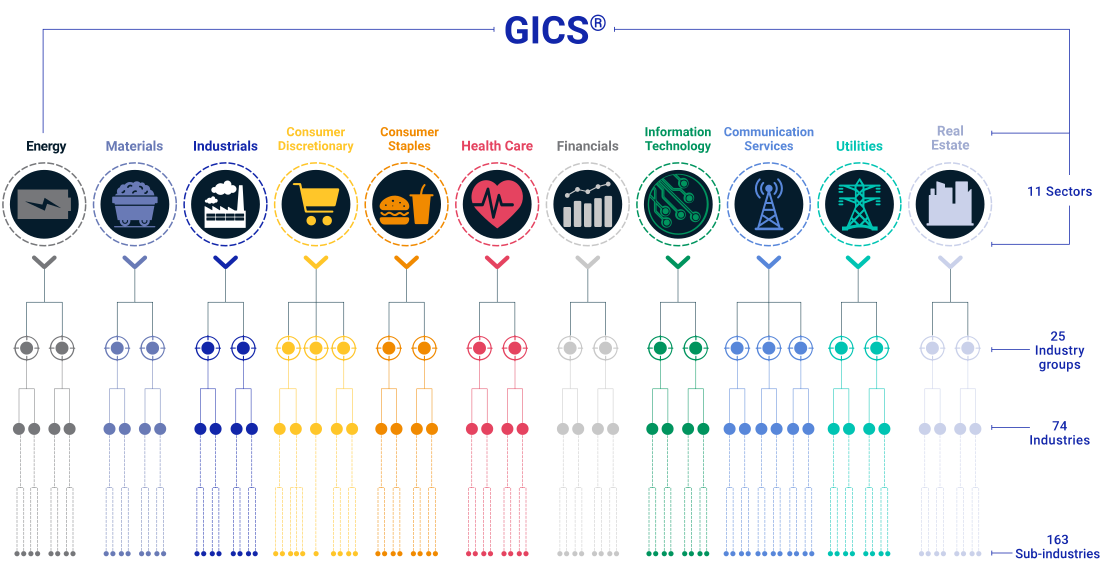
\includegraphics[width=5in]{figures/gics.png}
\caption{Global Industry Classification Standard (GICS) Structure \cite{GICS_MSCI}.}
\label{fig:label1}
\end{center}
\end{figure}


\newpage 
 \subsection{Data Cleaning Process Flowchart:}
\noindent This is a visual representation of the data cleaning process described in the data sources with a specification of the number of firm-years dropped at each step: 

\bigskip

\begin{figure}[H]
\centering
\begin{forest}
    for tree={
        draw,
        rounded corners,
        align=left,
        edge={->},
        parent anchor=south,
        child anchor=north,
        l sep+=0.5cm, % Increase the level distance
        scale=0.8,
    },
    [CDP Climate Response Survey Data\\\textbf{34,588 firm-years \& 11,289 firms}, fill=blue!20
        [Firm has an ISIN code?, edge, fill=yellow!20
            [\textbf{24,803 firm-years \& 4,330 firms}, edge label={node[midway, above left] {YES}}, fill=green!20
                [Is Worldscope + GICS data available?, edge, fill=yellow!20
                    [\textbf{19,200 firm-years \& 3,616 firms}, edge label={node[midway, above left] {YES}}, fill=green!20
                        [Is CDP control data available?, edge, fill=yellow!20
                            [\underline{\textbf{13,741 firm-years \& 3,574 firms}}, edge label={node[midway, above left] {YES}}, fill=green!20]
                            [\text{709} firm-years dropped, edge label={node[midway, above right] {NO}}, fill=red!20]
                        ]
                    ]
                    [\text{5,603} firm-years dropped, edge label={node[midway, above right] {NO}}, fill=red!20]
                ]
            ]
            [\text{9,785} firm-years dropped, edge label={node[midway, above right] {NO}}, fill=red!20]
        ]
    ]
\end{forest}
\captionof{table}{Data Cleaning Process Flowchart}
\label{fig:cdp-climate-response-survey-data}
\end{figure}

\noindent The final dataset contains \textbf{$\bf{18,476}$ firm-years across $\bf{3,574}$ firms, with complete CDP, Worldscope, and GICS data}. 
\newpage




\subsection{Variable Dictionary}

\noindent Table~\ref{tab:variable-dictionary} provides an overivew of the predictors used in the analysis, including their type, description, and source. Predictors are divided into three primary categories: \begin{itemize}
    \item \textbf{Firm Information:} Variables that describe the firm's characteristics, such as its unique identifier, reporting year, headquarters country, headquarters continent, and industry sector.
    \item \textbf{Financial Predictors:} Variables that capture the firm's financial performance, including total revenue, total assets, total employees, net income, and market capitalization.
    \item \textbf{CDP Predictors:} Variables derived from the CDP Climate Survey, such as the firm's emissions, energy consumption, and climate-related targets and initiatives.
\end{itemize}
\begin{longtable}{lp{2cm}p{6cm}p{2cm}} \\
    \toprule
    \textbf{Variable} & \textbf{Type} & \textbf{Description} & \textbf{Source} \\
    \midrule
    \endfirsthead % Everything above goes at the top of the first page of the table
    \multicolumn{4}{c}%
    {\tablename\ \thetable\ -- \textit{Continued from previous page}} \\
    \toprule
    \textbf{Variable} & \textbf{Type} & \textbf{Description} & \textbf{Source} \\
    \midrule
    \endhead % Header to be repeated on every page
    \bottomrule
    \multicolumn{4}{r}{\textit{Continued on next page}} \\
    \endfoot % Footer to be repeated on every page except the last
    \endlastfoot % Footer for the last page of the table
    
    % Core Information Section
    \multicolumn{4}{l}{\textbf{Firm Information}} \\
    \midrule
    ID & categorical & unique firm identifier & CDP \\
    Year & numerical & reporting year & CDP \\
    Country & categorical & headquarters country  & CDP \\
    Continent & categorical & headquarters continent derived from country & CDP \\
    Industry & categorical & Global Industry Classification Standard 25 industry sectors & GICS \\
    
    \midrule
    % Financial Predictors Section
    \multicolumn{4}{l}{\textbf{Financial Predictors}} \\
    \midrule
    log(Revenue) & numerical & natural logarithm of total revenue & Worldscope \\
    log(Assets) & numerical & natural logarithm of total assets & Worldscope \\
    log(Assets 1yr gr.) & numerical & natural logarithm of total assets growth & Worldscope \\
    log(Employees) & numerical & natural logarithm of total employees & Worldscope \\
    log(Empl. 1y gr.) & numerical & natural logarithm of total employees growth & Worldscope \\
    log(Net Income) & numerical & natural logarithm of net income & Worldscope \\
    log(Market Cap) & numerical & market capitalization & Worldscope \\
    log(Roe) & numerical & natural logarithm of return on equity & Worldscope \\
    log(Revenue) & numerical & natural logarithm of total revenue & Worldscope \\
    % Add more variables as needed
    \midrule
    % CDP Predictors Section
    \multicolumn{4}{l}{\textbf{CDP Predictors}} \\
    \midrule
    Variable5 & Type5 & Description5 & Source5 \\
    Variable6 & Type6 & Description6 & Source6 \\
    % Add more variables as needed
    
    \bottomrule
\caption{Variable Dictionary}
\label{tab:variable-dictionary}
\end{longtable}

\subsection{The Response Variable: Real Decarbonization Rate}

\begin{figure}[H]
    \begin{center}
    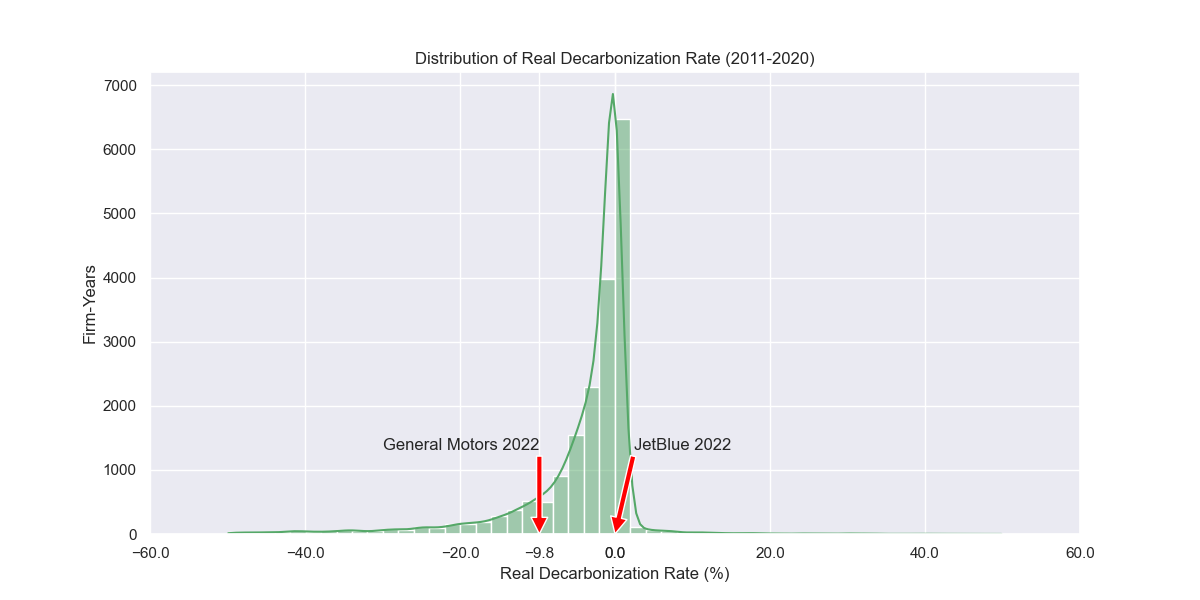
\includegraphics[width=5in]{figures/ghg_change_real_dist.png}
    \caption{Real Decarbonization Rate}
    \label{fig:real-decarbonization-rate}
    \end{center}
\end{figure}

\subsection{Real Decarbonization Rate Breakdown by Continent}
Figure \ref{fig:emission-breakdown-by-continent} and the relative table show the mean real decarbonization rate by continent across all CDP reporting years from 2011 to 2022. As expected, there is significant class imbalance between continents, with Europe having the most number of firms, followed by North America and Asia. There is a significant difference in the mean decarbonization rate across continents, with Europe having the best mean decarbonoization rate with an average yearly decrease of $-4.94 \%$ and Africa having the worst mean decarbonization rate with an average yearly decrease of $-2.81 \%$. Overall, the data suggests that operating in an environment with more incentives to report and reduce emissions, such as Europe, is associated with a higher mean decarbonization rate. This is consistent with the findings of Downar et al.  \cite{Downar2020The} which shows in a UK-based study that firms with a carbon disclosure mandate reduced emissions by $8\%$ without negatively impacting their financial operating performance. The hypothesis will be further tested in the following sections.
\noindent 

\begin{figure}[H]
    \begin{center}
    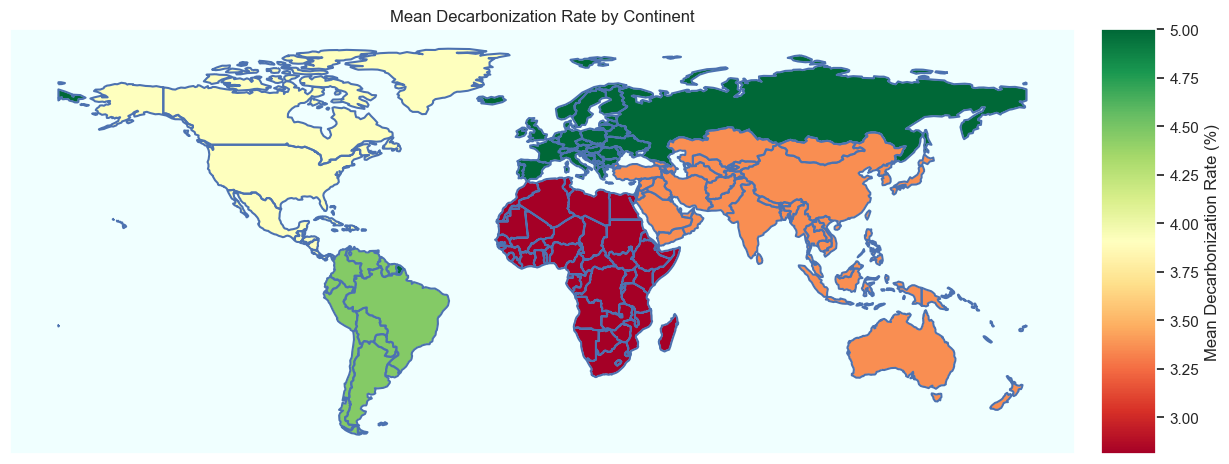
\includegraphics[width=5in]{figures/mean_decarbonization_rate_by_continent.png}
    \caption{Mean \textit{real decarbonization rate} by continent from 2011 to 2022}
    \label{fig:emission-breakdown-by-continent}
    \end{center}
\end{figure}
  

\begin{longtable}{lrlll}
\toprule
 & \# firms & Mean & Median & Std \\
Continent &  &  &  &  \\
\midrule
\endfirsthead
\toprule
 & \# firms & Mean & Median & Std \\
Continent &  &  &  &  \\
\midrule
\endhead
\midrule
\multicolumn{5}{r}{Continued on next page} \\
\midrule
\endfoot
\bottomrule
\endlastfoot
Africa & 79 & -2.8\% & -0.9\% & 5.9\% \\
Asia & 1175 & -3.1\% & -1.0\% & 6.4\% \\
Europe & 1217 & -4.9\% & -1.9\% & 8.6\% \\
North America & 933 & -3.5\% & -1.0\% & 7.3\% \\
Oceania & 101 & -3.1\% & -0.6\% & 6.9\% \\
South America & 90 & -4.0\% & 0.0\% & 10.1\% \\
\end{longtable}



\subsection{Real Decarbonization Rate Breakdown by Sector}

\noindent Figure \ref{fig:mean-decarbonization-rate-by-sector} and the relative table show the mean real decarbonization rate by sector across all CDP reporting years from 2011 to 2022. The data shows that the mean decarbonization rate varies significantly across sectors, with the best mean decarbonization rate in the Software and Services sector, with an average yearly decrease of $-6.67 \%$, and the worst mean decarbonization rate in the Materials sector, with an average yearly decrease of $-2.46\%$. Additionally, there are significant differences in the number of firms across sectors, with the Capital Goods sector having the most number of firms, $475$ and the Household and Personal Products sector having the least number of firms, $43$. Differences in sectors are important to consider, as they can be indicative of the difficulty of decarbonizing a given industry. For example, our data suggests that Transportation and Materials are the sectors with the worst mean decarbonization rates, which is consistent with the findings of Davis et al. \cite{Davis2018Net-zero} which suggest that difficult-to-decarbonize energy services include aviation, long-distance transport, steel and cement production.

\begin{figure}[H]
    \begin{center}
    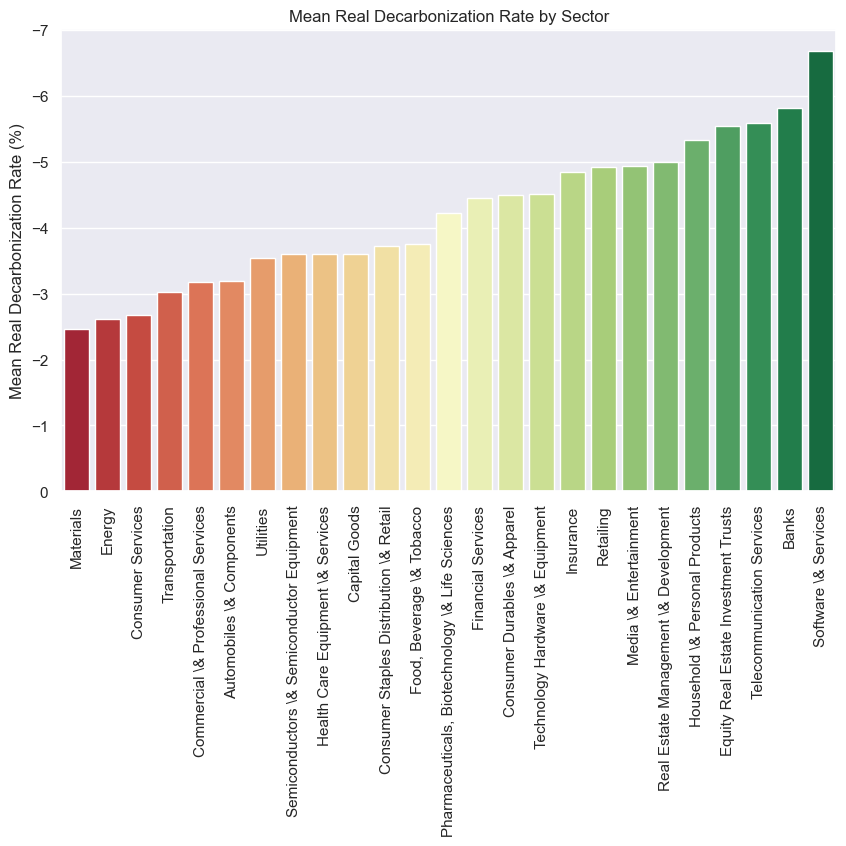
\includegraphics[width=5in]{figures/mean_decarbonization_rate_by_sector.png}
    \caption{Mean Real Decarbonization Rate by Sector}
    \label{fig:mean-decarbonization-rate-by-sector}
    \end{center}
\end{figure}


\begin{longtable}{lrlll}
\toprule
 & \# firms & Mean & Median & Std \\
Sector &  &  &  &  \\
\midrule
\endfirsthead
\toprule
 & \# firms & Mean & Median & Std \\
Sector &  &  &  &  \\
\midrule
\endhead
\midrule
\multicolumn{5}{r}{Continued on next page} \\
\midrule
\endfoot
\bottomrule
\endlastfoot
Automobiles \& Components & 124 & -3.2\% & -1.91\% & 5.54\% \\
Banks & 166 & -5.82\% & -2.9\% & 9.46\% \\
Capital Goods & 475 & -3.6\% & -1.1\% & 6.87\% \\
Commercial \& Professional Services & 134 & -3.18\% & -0.04\% & 7.7\% \\
Consumer Durables \& Apparel & 127 & -4.5\% & -1.4\% & 8.28\% \\
Consumer Services & 89 & -2.67\% & -0.96\% & 6.65\% \\
Consumer Staples Distribution \& Retail & 65 & -3.72\% & -1.9\% & 6.72\% \\
Energy & 151 & -2.62\% & -0.15\% & 5.66\% \\
Equity Real Estate Investment Trusts & 96 & -5.53\% & -2.33\% & 8.9\% \\
Financial Services & 158 & -4.45\% & -0.6\% & 8.98\% \\
Food, Beverage \& Tobacco & 187 & -3.75\% & -1.5\% & 6.63\% \\
Health Care Equipment \& Services & 100 & -3.6\% & -0.9\% & 7.45\% \\
Household \& Personal Products & 43 & -5.33\% & -2.4\% & 8.09\% \\
Insurance & 96 & -4.85\% & -2.0\% & 8.39\% \\
Materials & 420 & -2.46\% & -0.6\% & 5.78\% \\
Media \& Entertainment & 70 & -4.93\% & -0.54\% & 8.25\% \\
Pharmaceuticals, Biotechnology \& Life Sciences & 97 & -4.23\% & -1.8\% & 7.63\% \\
Real Estate Management \& Development & 53 & -4.99\% & -1.1\% & 8.86\% \\
Retailing & 115 & -4.93\% & -1.3\% & 9.43\% \\
Semiconductors \& Semiconductor Equipment & 79 & -3.6\% & -0.5\% & 8.15\% \\
Software \& Services & 140 & -6.67\% & -2.85\% & 10.21\% \\
Technology Hardware \& Equipment & 185 & -4.5\% & -1.8\% & 8.76\% \\
Telecommunication Services & 77 & -5.58\% & -2.34\% & 9.26\% \\
Transportation & 155 & -3.02\% & -1.0\% & 6.3\% \\
Utilities & 173 & -3.54\% & -0.1\% & 8.08\% \\
\end{longtable}
 

\subsection{Real Decarbonization Rate Breakdown by Country}

Figure \ref{fig:mean-decarbonization-rate-by-country} shows the mean real decarbonization rate by country across all CDP reporting years from 2011 to 2022. There are significant differences both in the number of firms and in the mean decarbonization rate across countries. Table~\ref{tab:emission_breakdown_country} shows summary statistics for the worst $10$ performing countries with nonzero mean real decarbonization rates. For a complete list of countries, see appendix table.


% include graph of mean decarbonization rates by country
\begin{figure}[htbp]
    \begin{center}
    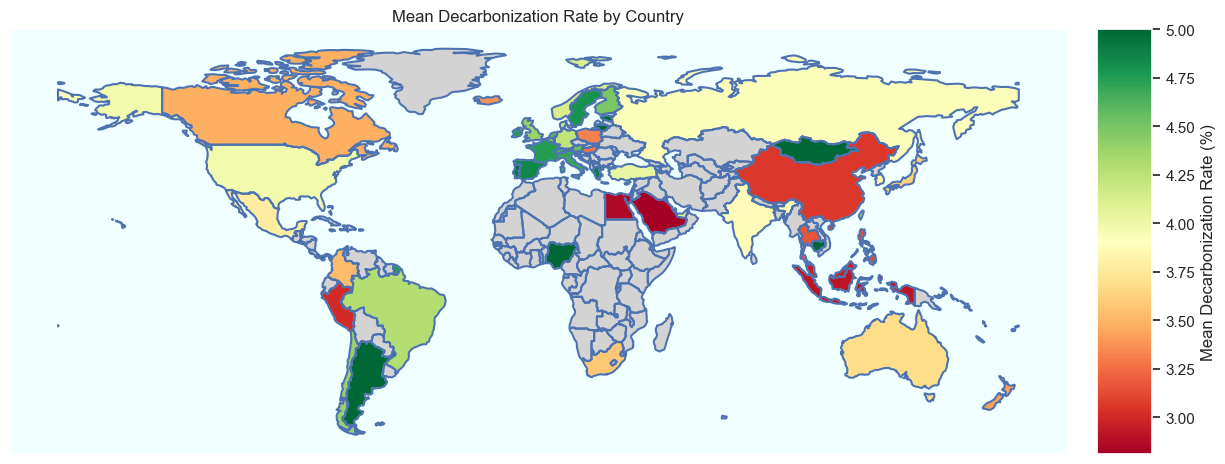
\includegraphics[width=5in]{figures/mean_decarbonization_rate_country.png}
    \caption{Mean Decarbonization Rate by Country}
    \label{fig:mean-decarbonization-rate-by-country}
    \end{center}
\end{figure}


\begin{longtable}{lrlll}
\toprule
 & \# firms & Mean & Median & Std \\
Country &  &  &  &  \\
\midrule
\endfirsthead
\toprule
 & \# firms & Mean & Median & Std \\
Country &  &  &  &  \\
\midrule
\endhead
\midrule
\multicolumn{5}{r}{Continued on next page} \\
\midrule
\endfoot
\bottomrule
\endlastfoot
Saudi Arabia & 1 & -0.6\% & -0.6\% & nan\% \\
Egypt & 2 & -1.46\% & 0.0\% & 2.85\% \\
Indonesia & 10 & -1.53\% & 0.0\% & 2.76\% \\
Malaysia & 13 & -1.57\% & 0.0\% & 6.19\% \\
Cayman Islands & 2 & -1.62\% & 0.0\% & 7.54\% \\
Peru & 1 & -1.67\% & 0.0\% & 4.53\% \\
China & 78 & -1.76\% & 0.0\% & 5.85\% \\
Hong Kong & 35 & -1.7\% & -0.27\% & 7.43\% \\
Philippines & 12 & -1.83\% & 0.0\% & 4.57\% \\
Thailand & 19 & -1.85\% & 0.0\% & 5.8\% \\
\caption{Emission Breakdown by Country}
\label{tab:emission_breakdown_country}
\end{longtable}


\subsection{Real Decarbonization Rate Breakdown by Year}

Figure \ref{fig:mean-decarbonization-rate-by-year} shows the mean and median real decarbonization rate by year across all CDP reporting years from 2011 to 2022. The data shows that the mean and median decarbonization rates have been (assuringly) decreasing over time.

\begin{figure}[H]
    \begin{center}
    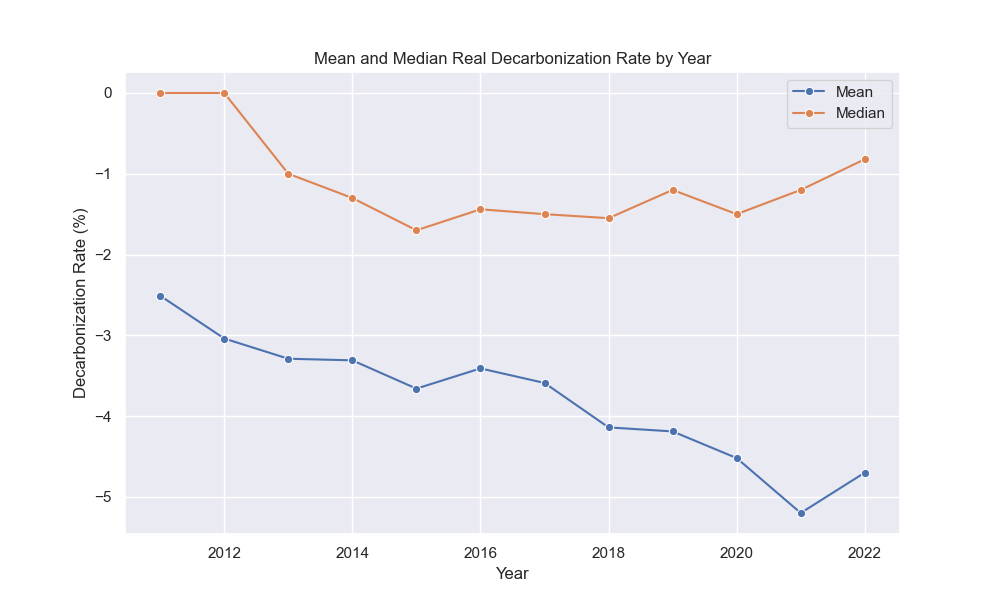
\includegraphics[width=5in]{figures/mean_decarbonization_rate_year.png}
    \caption{Mean and Median Real Decarbonization Rate by Year}
    \label{fig:mean-decarbonization-rate-by-year}
    \end{center}
\end{figure}

\begin{longtable}{lrlll}
\toprule
 & Count & Mean & Median & Std \\
Year &  &  &  &  \\
\midrule
\endfirsthead
\toprule
 & Count & Mean & Median & Std \\
Year &  &  &  &  \\
\midrule
\endhead
\midrule
\multicolumn{5}{r}{Continued on next page} \\
\midrule
\endfoot
\bottomrule
\endlastfoot
2011 & 1109 & -2.51\% & 0.0\% & 6.09\% \\
2012 & 1252 & -3.04\% & 0.0\% & 6.03\% \\
2013 & 1317 & -3.29\% & -1.0\% & 5.85\% \\
2014 & 1322 & -3.31\% & -1.3\% & 6.01\% \\
2015 & 1388 & -3.66\% & -1.7\% & 6.1\% \\
2016 & 1451 & -3.41\% & -1.44\% & 5.97\% \\
2017 & 1483 & -3.59\% & -1.5\% & 6.68\% \\
2018 & 1374 & -4.14\% & -1.55\% & 7.69\% \\
2019 & 1530 & -4.19\% & -1.2\% & 8.08\% \\
2020 & 1701 & -4.52\% & -1.5\% & 8.59\% \\
2021 & 2088 & -5.2\% & -1.2\% & 9.75\% \\
2022 & 2461 & -4.7\% & -0.82\% & 9.79\% \\
\caption{Real decarbonization rate by year}
\label{tab:real-decarbonization-rate-breakdown-by-year}
\end{longtable}



\subsection{Feature Engineering: Financial Predictors}
Figure \ref{fig:grid} shows the distribution of the financial predictors used in the analysis. This is a list of each predictor along with a brief description of how it was derived:
\begin{itemize}
    \item \textbf{Total Assets \ref{fig:total-assets}}: The total assets of the firm, which is a measure of the firm's size and the scale of its operations. Directly obtained from the Worldscope database and transformed using the natural logarithm $log(1 + \text{Total Assets})$.
    \item \textbf{Market Capitalization \ref{fig:market-capitalization}}: The market capitalization of the firm, which is a measure of the firm's size and the scale of its operations. Directly obtained from the Worldscope database and transformed using the natural logarithm $log(1 + \text{Market Cap})$.
    \item \textbf{Return on Equity \ref{fig:roe}}: The return on equity of the firm, which is a measure of the firm's profitability. Since the return on equity is a percentage which can be negative, the following transformation was used: $log(1 + \frac{\text{ROE}}{100})$.
    \item \textbf{Revenue \ref{fig:revenue}}: The total revenue of the firm, which is a measure of the firm's size and the scale of its operations. Directly obtained from the Worldscope database and transformed using the natural logarithm $log(1 + \text{Revenue})$.
    \item \textbf{Net Income \ref{fig:net-income}}: The net income of the firm, which is a measure of the firm's profitability. Directly obtained from the Worldscope database and transformed using the natural logarithm $log(1 + \text{Net Income})$.
    \item \textbf{Employees \ref{fig:employees}}: The total number of employees of the firm, which is a measure of the firm's size and the scale of its operations. Directly obtained from the Worldscope database and transformed using the natural logarithm $log(1 + \text{Employees})$.
    \item \textbf{Total Assets 1yr Growth \ref{fig:total-assets-1yr-growth}}: The one year growth of the total assets of the firm, which is a measure of the firm's growth. Directly obtained from the Worldscope database and since the growth can be negative, the following transformation was used: $log(1 + \frac{\text{Total Assets 1yr Growth}}{100})$.
    \item \textbf{Employees 1yr Growth \ref{fig:employees-1yr-growth}}: The one year growth of the total number of employees of the firm, which is a measure of the firm's growth. Directly obtained from the Worldscope database and since the growth can be negative, the following transformation was used: $log(1 + \frac{\text{Employees 1yr Growth}}{100})$.
    \item \textbf{Net Income over Assets \ref{fig:net-income}}: The net income of the firm over its total assets, which is a measure of the firm's profitability. The feature was calculated with the following formula $log(1 + \frac{\text{Net Income}}{\text{Total Assets}})$.
\end{itemize}

\begin{figure}[H]
\centering

% Row 1
\subcaptionbox{Total Assets\label{fig:total-assets}}{%
  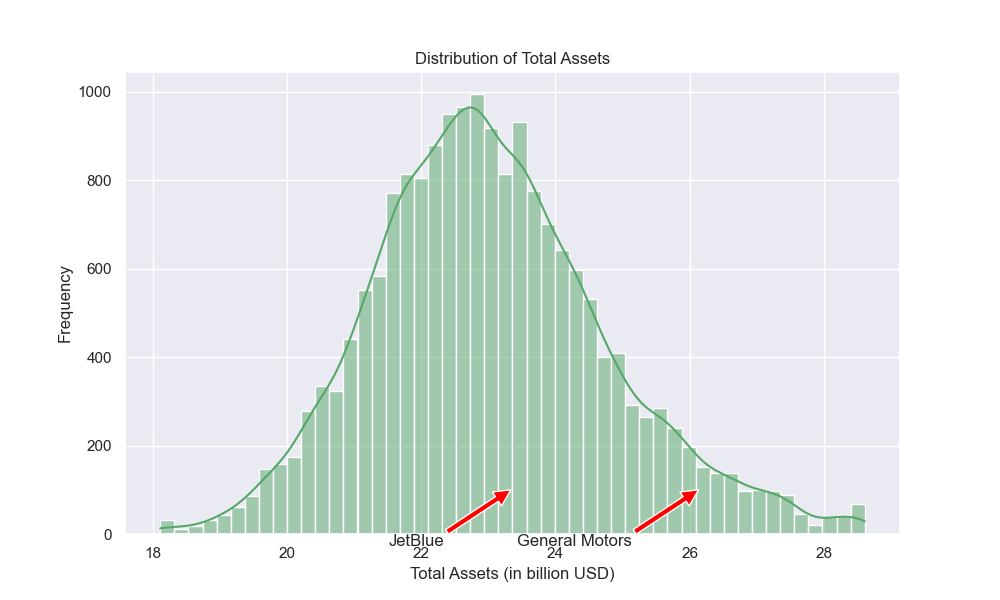
\includegraphics[width=0.3\linewidth]{figures/financial_preds/tot_assets_dist.png}}%
\hfill % spacing between images
\subcaptionbox{Market Capitalization\label{fig:market-capitalization}}{%
  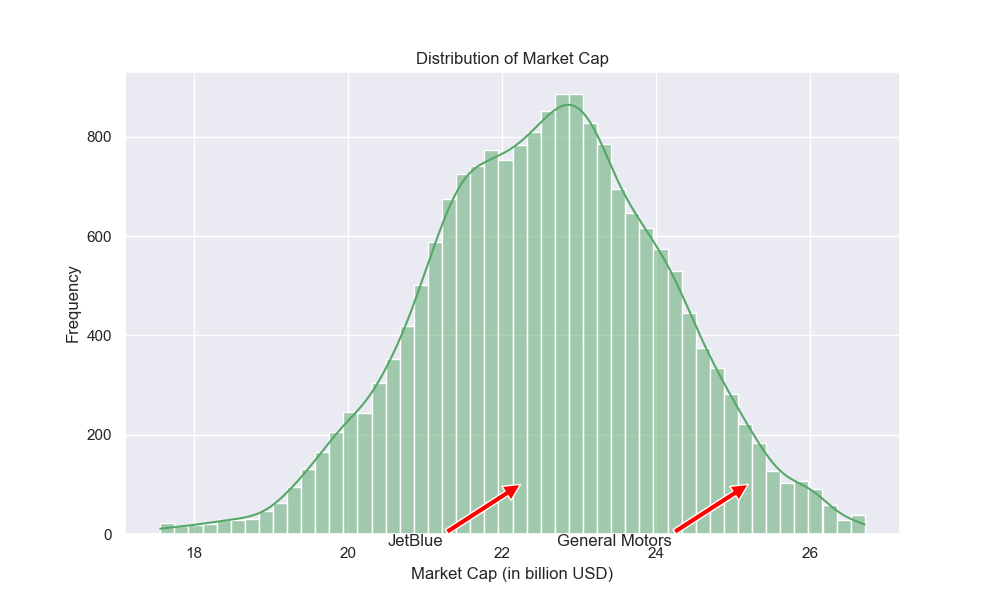
\includegraphics[width=0.3\linewidth]{figures/financial_preds/mkt_cap_dist.png}}%
\hfill % spacing between images
\subcaptionbox{Return on Equity\label{fig:roe}}{%
  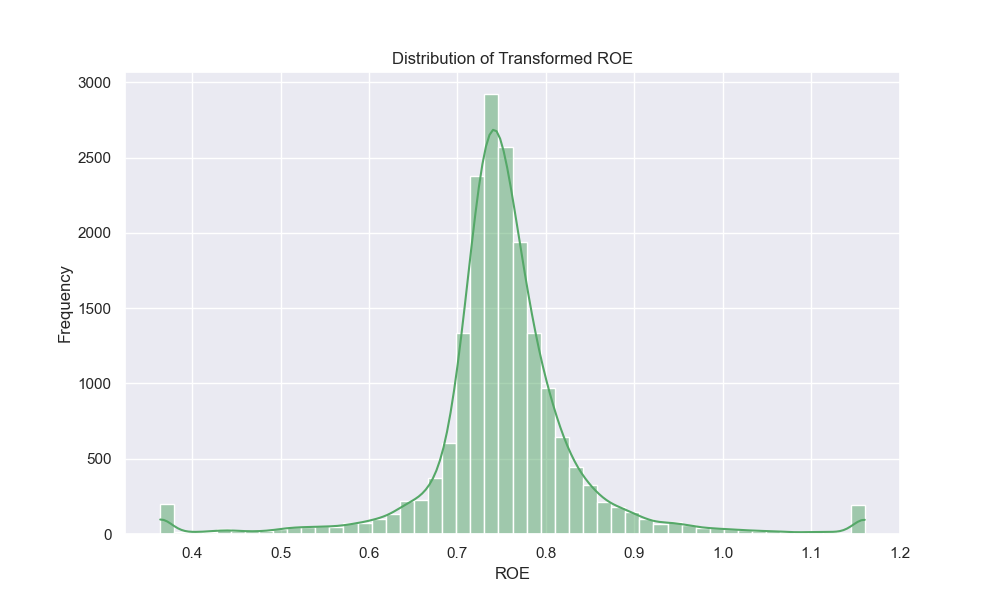
\includegraphics[width=0.3\linewidth]{figures/financial_preds/roe_dist.png}}%

% Row 2
\subcaptionbox{Revenue\label{fig:revenue}}{%
  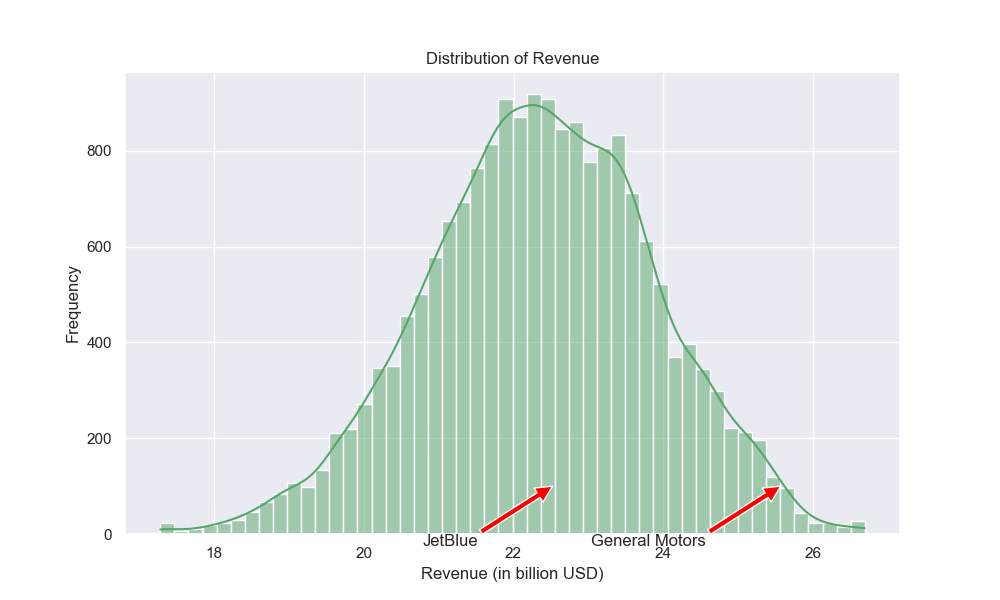
\includegraphics[width=0.3\linewidth]{figures/financial_preds/revenue_dist.png}}%
\hfill
\subcaptionbox{Net Income\label{fig:net-income}}{%
  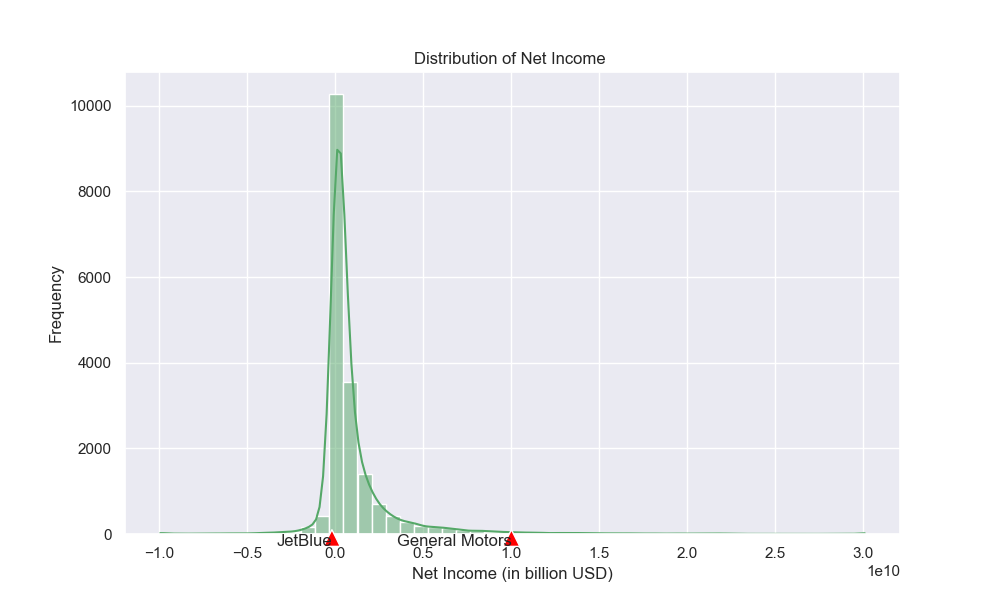
\includegraphics[width=0.3\linewidth]{figures/financial_preds/net_income_dist.png}}%
\hfill
\subcaptionbox{Employees\label{fig:employees}}{%
  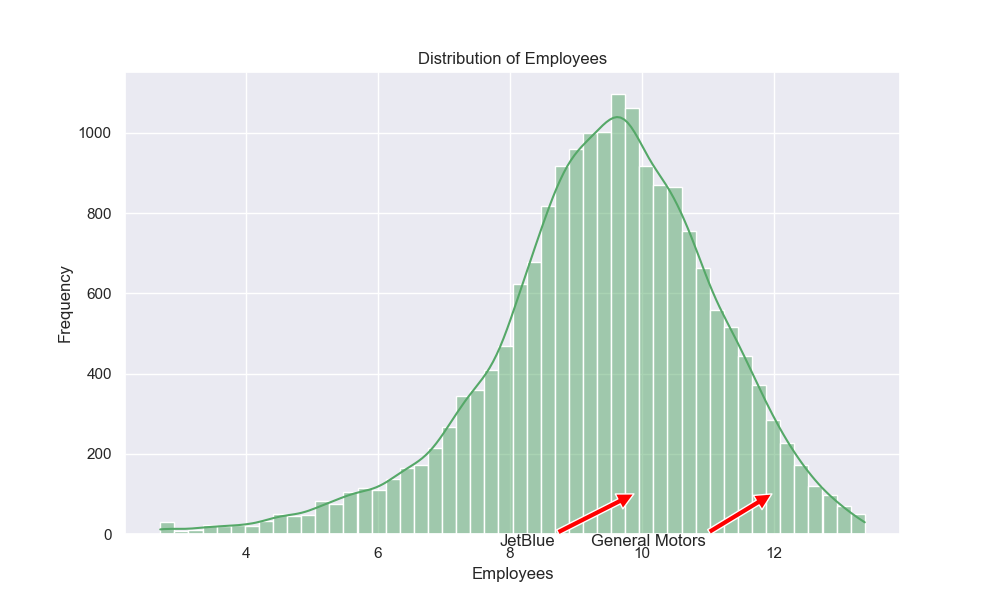
\includegraphics[width=0.3\linewidth]{figures/financial_preds/employees_dist.png}}%

% Row 3
\subcaptionbox{Tot. Assets 1yr Growth\label{fig:total-assets-1yr-growth}}{%
  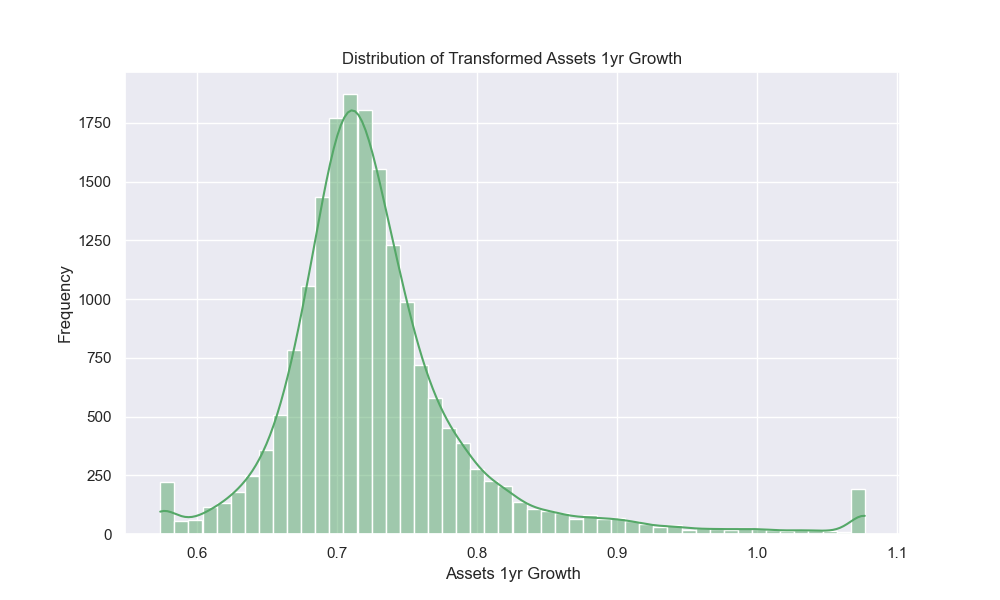
\includegraphics[width=0.3\linewidth]{figures/financial_preds/assets_1yr_growth_dist.png}}%
\hfill % spacing between images
\subcaptionbox{Employees 1yr Growth\label{fig:employees-1yr-growth}}{%
  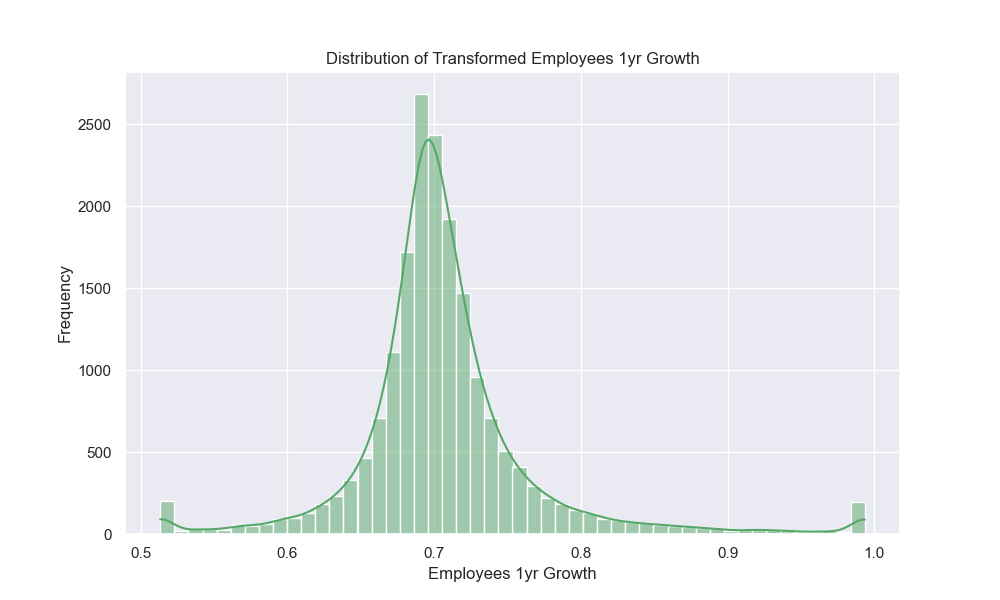
\includegraphics[width=0.3\linewidth]{figures/financial_preds/employees_1yr_growth_dist.png}}%
\hfill % spacing between images
\subcaptionbox{Net Income Over Assets\label{fig:net-income-over-assets}}{%
  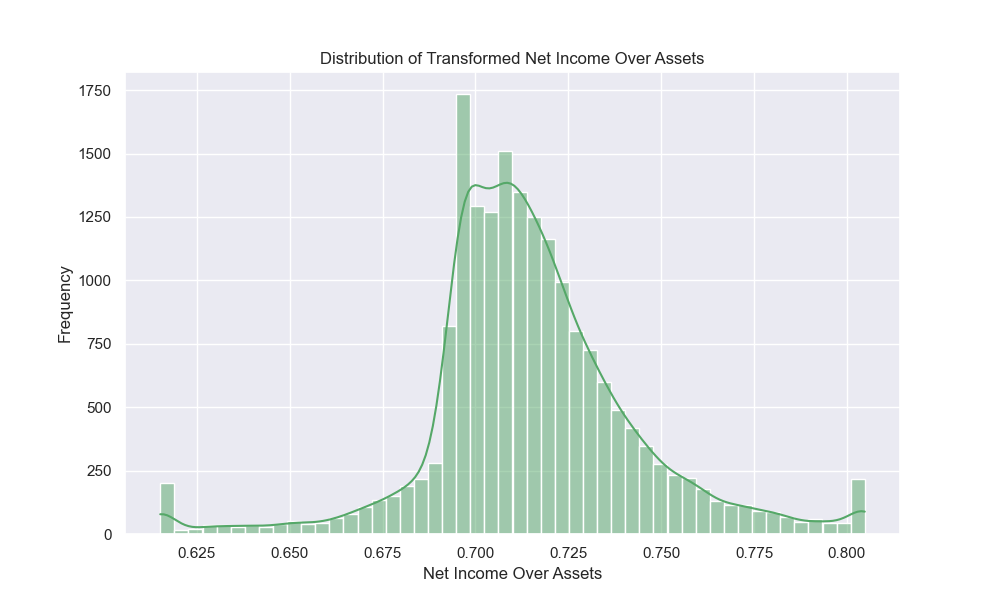
\includegraphics[width=0.3\linewidth]{figures/financial_preds/net_income_over_assets_dist.png}}%



\caption{Financial Predictors}
\label{fig:grid}
\end{figure}

\noindent \textit{Note: for full-size images, see appendix \ref{sec:FinancialPreds}.}
\newpage 

\begin{itemize}
    \item Number of firms and unique isins
    \item Number of variables
    \item Number of firms per sector
\end{itemize}